\documentclass[compress]{beamer}
\usepackage{irbookslide}
\usepackage{irilmenau2}
\usepackage{tikz}
\usepackage{url}
\usepackage{ifxetex}
%\RequireXeTeX
\usepackage{fontspec} % zahteva paket euenc
\usepackage{xunicode}
\usepackage{xltxtra}
\usepackage{polyglossia}
\usepackage{minted}
\usepackage{algorithmic}
\renewcommand{\algorithmicrequire}{\textbf{Input:}}
\renewcommand{\algorithmicensure}{\textbf{Output:}}
\usepackage{xcolor,colortbl}
\usepackage{textcomp}
%\setdefaultlanguage[script=Latin]{serbian}

\title{Redovi}
\author{\textcopyright \ \ Goodrich, Tamassia, Goldwasser}
\institute{Katedra za informatiku, Fakultet tehničkih nauka, Univerzitet u
Novom Sadu}
\date{2014.}
\subject{Predavanja sa ASP}

\begin{document}

\frame{\titlepage}

\section[Pojam reda]{Pojam reda}
\begin{frame}[fragile]
  \frametitle{Red ATP}
  \begin{itemize}
    \item \myred{red} (queue) ATP čuva proizvoljne objekte
    \item ubacivanje i uklanjanje poštuje FIFO (first-in-first-out) princip
    \item ubacivanje se vrši na kraju reda, a uklanjanje na početku reda
    \item glavne operacije:
    \begin{itemize}
      \item \myred{enqueue}(object): dodaje element na kraj reda
      \item object \myred{dequeue}(): uklanja element sa početka reda
    \end{itemize}
    \item dodatne operacije:
    \begin{itemize}
      \item object \myred{first}(): vraća element sa početka bez uklanjanja
      \item integer \myred{len}(): vraća broj elemenata u redu
      \item boolean \myred{is\_empty}(): vraća True ako je red prazan
    \end{itemize}
    \item greške:
    \begin{itemize}
      \item poziv \myred{dequeue} ili \myred{first} za prazan red
    \end{itemize}
  \end{itemize}
\end{frame}

\begin{frame}[fragile,shrink=10]
  \frametitle{Primer operacija nad redom}
\begin{center}
\begin{tabular}{lcl}
\textbf{operacija} & \textbf{rezultat} & \textbf{sadržaj reda} \\
\hline \hline
\texttt{Q.enqueue(5)} & -- & [5] \\ 
\texttt{Q.enqueue(3)} & -- & [5,3] \\ 
\texttt{len(Q)} & 2 & [5,3] \\ 
\texttt{Q.dequeue()} & 5 & [3] \\ 
\texttt{Q.is\_empty()} & False & [3] \\ 
\texttt{Q.dequeue()} & 3 & [] \\ 
\texttt{Q.is\_empty()} & True & [] \\ 
\texttt{Q.dequeue()} & greška & [] \\ 
\texttt{Q.enqueue(7)} & -- & [7] \\ 
\texttt{Q.enqueue(9)} & -- & [7,9] \\ 
\texttt{Q.first()} & 7 & [7,9] \\ 
\texttt{Q.enqueue(4)} & -- & [7,9,4] \\ 
\texttt{len(Q)} & 3 & [7,9,4] \\ 
\texttt{Q.dequeue()} & 7 & [9,4] \\ 
\end{tabular}
\end{center}
\end{frame}

\begin{frame}[fragile]
  \frametitle{Primene redova}
  \begin{itemize}
    \item neposredne primene
    \begin{itemize}
      \item liste čekanja, birokratija
      \item pristup deljenim resursima (npr. štampač)
      \item deljenje procesora među paralelnim procesima
    \end{itemize}
    \item indirektne primene
    \begin{itemize}
      \item pomoćna struktura podataka za mnoge algoritme
      \item komponenta u okviru drugih struktura podataka
    \end{itemize}
  \end{itemize}
\end{frame}

\begin{frame}[fragile]
  \frametitle{Red pomoću niza}
  \begin{itemize}
    \item implementiraćemo stek pomoću niza dužine $N$
    \item koristimo ga cirkularno
    \item posebna promenljive čuvaju indekse prvog i poslednjeg elementa
    \begin{itemize}
      \item $f$ -- indeks prvog elementa
      \item $r$ -- indeks prvog elementa iza od poslednjeg
    \end{itemize}
    \item element niza sa indeksom $r$ je uvek prazan!      
  \end{itemize}
  \begin{center}
    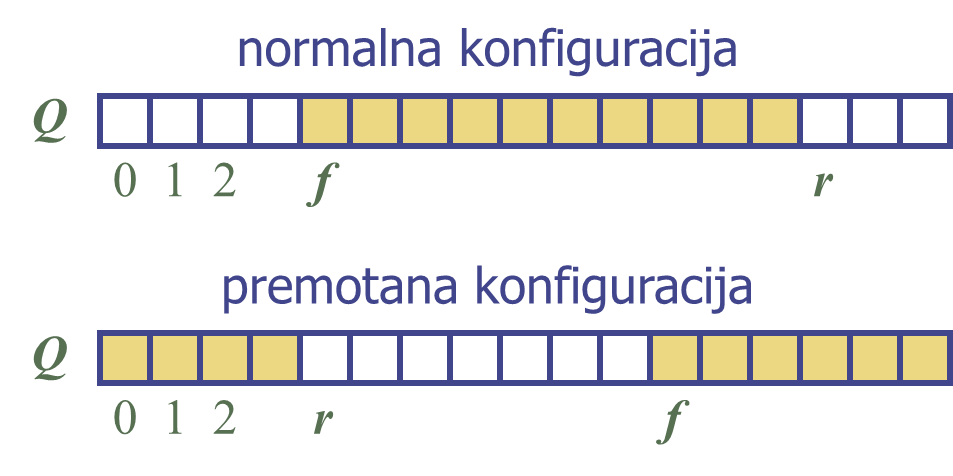
\includegraphics[width=8cm]{asp-06-pic01.png}
  \end{center}
\end{frame}

\begin{frame}[fragile]
  \frametitle{Red pomoću niza $_2$}
  \begin{itemize}
    \item koristićemo moduo operator (ostatak pri deljenju)
    \item broj elemenata reda i test da li je prazan:
  \end{itemize}
\myred{size}()
\begin{algorithmic}
\RETURN $(N-f+r) \mod N$
\end{algorithmic}
\\ \ \\
\myred{isEmpty}()
\begin{algorithmic}
\RETURN $(f=r)$
\end{algorithmic}
\begin{center}
  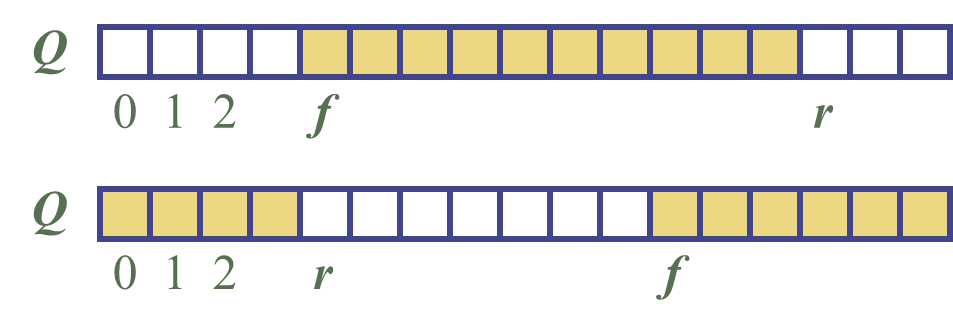
\includegraphics[width=8cm]{asp-06-pic02.png}
\end{center}
\end{frame}

\begin{frame}[fragile]
  \frametitle{Red pomoću niza $_3$}
  \begin{itemize}
    \item operacija \myred{enqueue} izaziva izuzetak ako je niz pun
  \end{itemize}
\myred{enqueue}($e$)
\begin{algorithmic}
\IF{size()$=N-1$}
  \STATE throw FullQueueException
\ELSE
  \STATE $Q[r] \leftarrow e$
  \STATE $r \leftarrow (r+1)\mod N$
\ENDIF
\end{algorithmic}
\begin{center}
  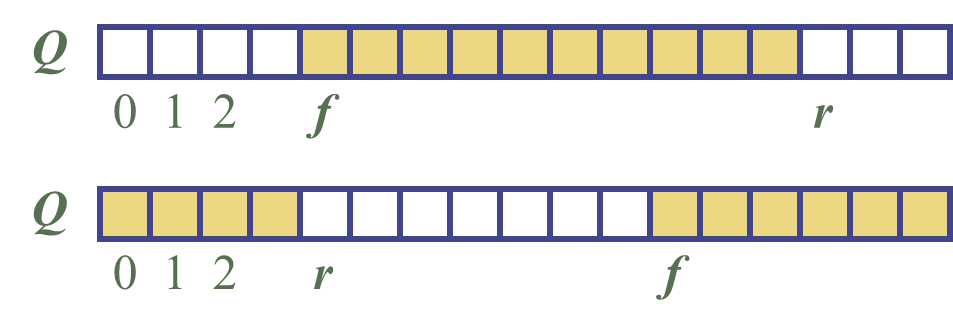
\includegraphics[width=8cm]{asp-06-pic02.png}
\end{center}
\end{frame}

\begin{frame}[fragile]
  \frametitle{Red pomoću niza $_4$}
  \begin{itemize}
    \item operacija \myred{dequeue} izaziva izuzetak ako je red prazan
  \end{itemize}
\myred{dequeue}()
\begin{algorithmic}
\IF{isEmpty()}
  \STATE throw EmptyQueueException
\ELSE
  \STATE $e \leftarrow Q[f]$
  \STATE $f \leftarrow (f+1)\mod N$
  \RETURN $e$
\ENDIF
\end{algorithmic}
\begin{center}
  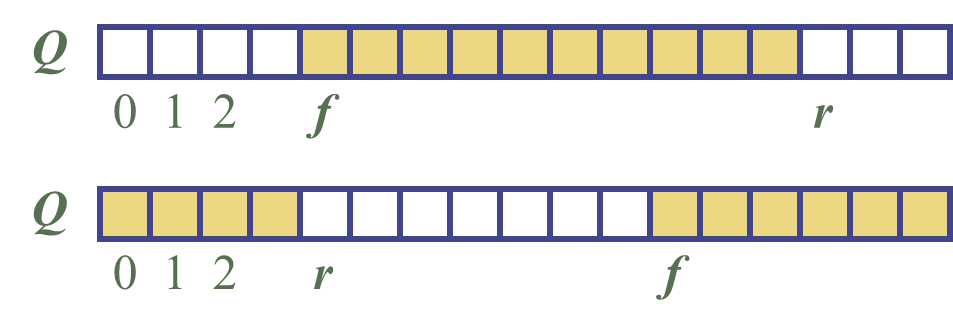
\includegraphics[width=8cm]{asp-06-pic02.png}
\end{center}
\end{frame}

\section[Python impl]{Implementacija u Pythonu}
\begin{frame}[fragile]
  \frametitle{Implementacija reda u Pythonu}
  \begin{itemize}
    \item imaćemo tri atributa:
    \item \texttt{\_data}: lista sa fiksnim kapacitetom
    \item \texttt{\_size}: broj elemenata u redu
    \item \texttt{\_front}: indeks prvog elementa u redu
  \end{itemize}
\end{frame}

\begin{frame}[fragile,shrink=10]
  \frametitle{Implementacija reda u Pythonu $_1$}
\begin{minted}[linenos=false]{python}
class ArrayQueue:
  DEFAULT_CAPACITY = 10

  def __init__(self):
    self._data = [None] * DEFAULT_CAPACITY
    self._size = 0
    self._front = 0
    
  def __len__(self):
    return self._size
  
  def is_empty(self):
    return self._size == 0
    
  def first(self):
    if self.is_empty():
      raise Empty('queue is empty')
    return self._data[self._front]

  def dequeue(self):
    if self.is_empty():
      raise Empty('queue is empty')
    answer = self._data[self._front]
    self._data[self._front] = None
    self._front = (self._front + 1) % len(self._data)
    self.size -= 1
    return answer
\end{minted}
\end{frame}

\begin{frame}[fragile,shrink=10]
  \frametitle{Implementacija reda u Pythonu $_2$}
\begin{minted}[linenos=false]{python}
  def enqueue(self, e):
    if self._size == len(self._data):
      self._resize(2*len(self.data))
    avail = (self._front + self._size) % len(self._data)
    self._data[avail] = e
    self._size += 1
    
  def _resize(self, cap):
    old = self._data
    self._data = [None] * cap
    walk = self._front
    for k in range(self._size):
      self._data[k] = old[walk]
      walk = (1 + walk) % len(old)
    self._front = 0 
\end{minted}
\end{frame}

\section[P: Round Robin]{Primer: round robin raspoređivanje}
\begin{frame}[fragile]
  \frametitle{Round robin raspoređivanje}
  \begin{itemize}
    \item obrada zahteva u krug
    \item[1] $e \leftarrow Q$.dequeue()
    \item[2] obradi $e$
    \item[3] $Q$.enqueue($e$)
  \end{itemize}
\begin{center}
  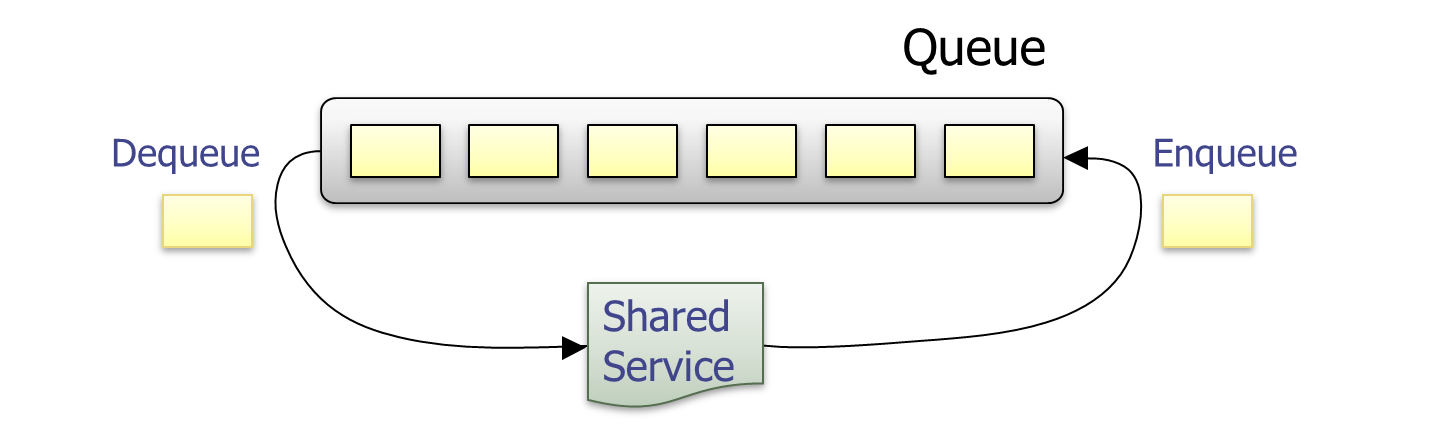
\includegraphics[width=10cm]{asp-06-pic03.png}
\end{center}
\end{frame}

\end{document}
